\documentclass[a4paper, 11pt, titlepage]{article}
\usepackage{graphicx}
\usepackage{pdfpages}
\usepackage{fancybox}
\usepackage[english]{babel}
\usepackage[utf8]{inputenc}
% \usepackage[T1]{fontenc}
\usepackage{amsmath,amsfonts,amssymb}
\usepackage{fancyhdr}
\usepackage{stackrel}
\usepackage{babel,indentfirst}
\usepackage{xspace}
\usepackage{url}
\usepackage{titling}
\usepackage{listings}
\usepackage{color}
\usepackage{array}
\usepackage{hyperref}
\usepackage{makecell}
\usepackage{tikz}
\usepackage{float}
\usepackage{wrapfig}

%\setlength{\parindent}{0pt}
\setlength{\parskip}{1ex}
\setlength{\textwidth}{17cm}
\setlength{\textheight}{24cm}
\setlength{\oddsidemargin}{-.7cm}
\setlength{\evensidemargin}{-.7cm}
\setlength{\topmargin}{-.5in}


\lstset{
  sensitive=f,
  morestring=[d]",
  showstringspaces=false,
  basicstyle=\small\ttfamily,
  keywordstyle=\bf\small,
  commentstyle=\itshape,
  stringstyle=\sf,
  extendedchars=true,
  columns=[c]fixed
}



\predate{
\begin{center}
}
\postdate{
\\
\vspace{1.5cm}

\includegraphics[scale=0.7]{imag.png}
\end{center}}


\title {{ {\huge NoSQL project report }} }

\author{\Large Team 7 \\
\\
    {\sc Bouchoux}~Adrien\\
    {\sc Gouttefarde}~Léo\\
    {\sc Nahyl}~Othmane
}

\date{Wednesday 14th December 2016}

\lhead{NoSQL project}
\rhead{Report}

\begin{document}
\pagestyle{fancy}
\maketitle

\setcounter{tocdepth}{2}

\tableofcontents
\newpage


% \begin{center}
% \section* {Introduction}
% \end{center}

\section {NoSQL system choice}

For this project, we chose the Neo4j system.


\section {Data stored in the database}

% Write a text describing the data stored in the database. This text should not exceed 15 lines. You can include a figure to illustrate.

The database describes relationships between persons and companies established in several industries. Each person has a name and a birth date attribute. A person can have several skills with a specific level, and lives in a country (whose only attribute is the name of the country). Any person can also be an employee, ending up having 2 labels.

A company has a name as attribute, and is specialized in one or several industries (eg. Oil, Farming, …) and established in one or several countries.
Some companies are looking for specific skills. Every employee may work in a company. In this case, the start date and the salary can be stored in the relation between the person and the company.

Persons may know each other. The relationship level can be stored as a relation property.

For more informations, please look at the figure bellow :


\begin{center}
% % \begin{figure}[ht!]
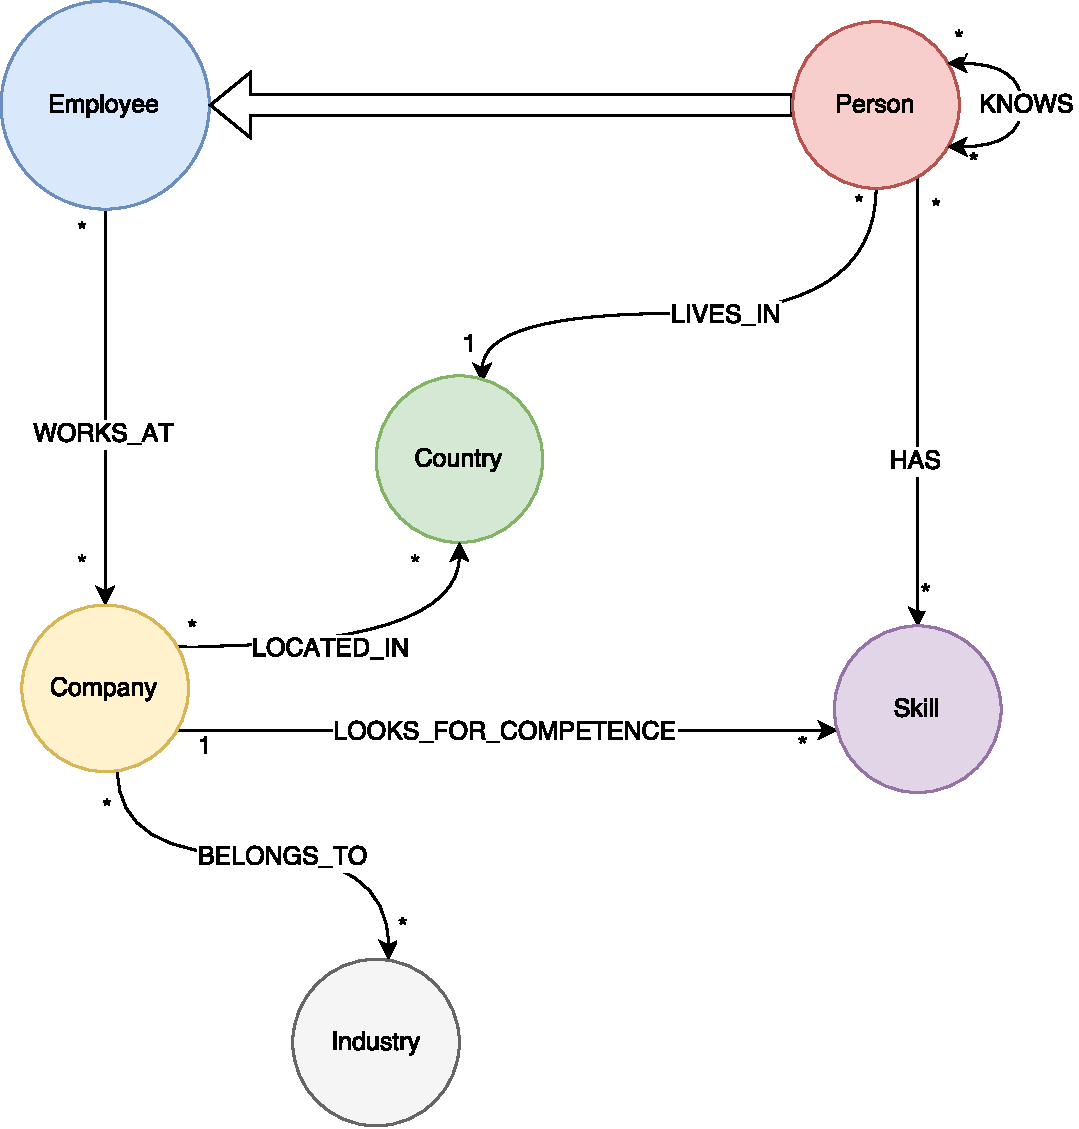
\includegraphics[scale=0.6]{res/database.pdf}
% % \caption{Diagramme de classes du modèle}
% % \end{figure}
\end{center}


\section {Indexes}

%=> Describe the indexes proposed and explain your decision. This text should not exceed 4 lines by index.

We use an index on each node type's name property, and another index for the birth date in nodes of type Person. Indeed we use a name attribute on each node type to identify every instance, therefore an index will speed up identification requests a lot.


\section {Queries}

\subsection {Query 1}

\subsection* {Description}

\noindent
This query retrieves companies and the number of experts and intermediates (all skills included) that they are looking for.


\subsection* {Code}

\begin{verbatim}
MATCH (cmp:Company)-[r:LOOKS_FOR_COMPETENCE]->(s:Skill)
MATCH (company_country:Country)<-[]-(cmp)
MATCH (prs:Person)-[h:HAS]->(s)
MATCH (person_country:Country)<-[]-(prs)
WHERE h.level IN ['Intermediate', 'Expert'] 
AND person_country.name = company_country.name
RETURN cmp AS Company, count(prs) AS Number;
\end{verbatim}


\subsection* {Index impact}

\noindent
The number of country nodes compared by name will be reduced thanks to the index on the country name property.



\subsection* {Advantages and disadvantages of this implementation}

\noindent
The different MATCH layers allow us to filter the different nodes before applying the last query layer with the two comparisons. The index on the name property helps ignoring some data.

\noindent
This implementation is good because all used properties are indexed correctly, bringing excellent performance. No specific disadvantage appears here.





\subsection {Query 2}

\subsection* {Description}

\noindent
For the Apple company, get the list of persons who have an affinity with somebody working in the same company, and who have at least one skill of the same level in common with the latter.


\subsection* {Code}

\begin{verbatim}
MATCH (c:Company {name: 'Apple'})-[WORKS_AT]-(e:Employee)-[KNOWS]-(ee:Employee)
MATCH (s:Skill)<-[h:HAS]-(e)
OPTIONAL MATCH (ss:Skill)<-[hh:HAS]-(ee)-[WORKS_AT]-(c)
WHERE h.level = hh.level
RETURN ee AS Employee;
\end{verbatim}


\subsection* {Index impact}

\noindent
The index established on the name of the company reduces the number of nodes retrieved by the first MATCH part of the query.



\subsection* {Advantages and disadvantages of this implementation}

\noindent
The index enables to ignore inconsistent data such as people working in other companies. The filtering of nodes at the first line reduces the amount of nodes and as a result the number of comparisons executed.

\noindent
A disadvantage however, is that the level attributes have to be compared as strings for each matching pair of Person nodes. Unnecessary nodes can be matched.


\subsection {Query 3}

\subsection* {Description}

\noindent
Retrieve the list of companies working in 'Software Engineering' and 'Oil' who employ persons specialised in 'Finance'.


\subsection* {Code}

\begin{verbatim}
MATCH (ss:Skill {name: 'Finance'})-[HAS]-(ee:Person:Employee)-
[WORKS_AT]-(cc:Company)-[BELONGS_TO]-(ii:Industry {name: 'Software Engineering'})
OPTIONAL MATCH (cc)-[BELONGS_TO]-(jj:Industry {name: 'Oil'})
RETURN cc AS Company;
\end{verbatim}


\subsection* {Index impact}

\noindent
The created indexes allow to speed up name matching for the Skill, Industry and second Industry nodes in the MATCH commands.


\subsection* {Advantages and disadvantages of this implementation}

\noindent
This implementation is good because all used properties are indexed correctly, bringing excellent performance. No specific disadvantage appears here.


\subsection {Query 4}

\subsection* {Description}

\noindent
Increase by 200 \% the salary of all employees experts in 'Neo4j' for 'Software Engineering' companies.


\subsection* {Code}

\begin{verbatim}
MATCH (ss:Skill {name: 'Neo4j'})-[HAS {level: 'Expert'}]-(ee:Person:Employee)-
[ww:WORKS_AT]-(cc:Company)-[BELONGS_TO]-(ii:Industry {name: 'Software Engineering'})
SET ww.salary = 3 * ww.salary;
\end{verbatim}


\subsection* {Index impact}

\noindent
The created indexes allow to speed up name matching for the Skill and Industry nodes.


\subsection* {Advantages and disadvantages of this implementation}

\noindent
This implementation uses several indexes, which brings good speed up in performance. However the skill relationship level property is a non indexed string element, therefore there may be a better way to do that part efficiently.



\subsection {Query 5}

\subsection* {Description}

\noindent
Fire (delete the work relationship) all employees in finance who have a beginner level in all of their skills or no skill at all.


\subsection* {Code}

\begin{verbatim}
MATCH (bb:Skill)-[HAS {level: 'Beginner'}]-(ee:Employee)-
[ww:WORKS_AT]-(cc:Company)-[BELONGS_TO]-(ii:Industry {name: 'Finance'})
OPTIONAL MATCH (ee)-[HAS]-(ss:Skill)
WITH ww, count(bb) AS bbCount, count(ss) AS ssCount
WHERE bbCount = ssCount
DELETE ww;
\end{verbatim}


\subsection* {Index impact}

\noindent
The created indexes allow to speed up name matching for the Industry node, which brings some better performance.


\subsection* {Advantages and disadvantages of this implementation}

\noindent
This implementation is still good because it uses an index on the Industry name matching. However the skill relationship level property is a non indexed string element, therefore there may be a better way to do that part efficiently.



\end{document}


